\documentclass[
	aspectratio=169, % default is 43
	8pt, % font size, default is 11pt
	%handout, % handout mode without animations, comment out to add animations
]{beamer}

\usepackage{../template/beamerthemeuulm} % use the inofficial uulm beamer theme
\usepackage[ngerman]{babel} % use this line for slides in German
%\usepackage{minted} % for displaying source code

\usepackage{tabularx}

\usepackage{listings}
\usepackage{color} %red, green, blue, yellow, cyan, magenta, black, white
\definecolor{mygreen}{RGB}{28,172,0} % color values Red, Green, Blue
\definecolor{mylilas}{RGB}{170,55,241}
\lstset{language=Matlab,%
    %basicstyle=\color{red},
    breaklines=true,%
    morekeywords={matlab2tikz},
    keywordstyle=\color{blue},%
    morekeywords=[2]{1}, keywordstyle=[2]{\color{black}},
    identifierstyle=\color{black},%
    stringstyle=\color{mylilas},
    commentstyle=\color{mygreen},%
    showstringspaces=false,%without this there will be a symbol in the places where there is a space
    numbers=left,%
    numberstyle={\tiny \color{black}},% size of the numbers
    numbersep=9pt, % this defines how far the numbers are from the text
    emph=[1]{for,end,break},emphstyle=[1]\color{red}, %some words to emphasise
    %emph=[2]{word1,word2}, emphstyle=[2]{style},    
}

\graphicspath{{./pics/}{../template/pics/}{../template/pics/logos/}{../template/pics/uulm/}{../template/pics/nature/}} % set the path for images and logos

% Colors:
%\definecolor{sfzgreen}{HTML}{79bf38}
%\definecolor{sfzpurple}{HTML}{5c64b8}
%\definecolor{sfzgray}{HTML}{acacaa}

%\definecolor{red}{HTML}{A32638} % sfz-red
%\definecolor{orange}{HTML}{79bf38} % sfz-green
%\definecolor{blue}{HTML}{5c64b8} % sfz-purple

%\setbeamercolor{myfooter}{fg=white,bg=sfzgray}
%\setbeamercolor{subtitlebox}{fg=white,bg=sfzgray}
%\setbeamercolor{mypagenumber}{fg=white,bg=sfzgreen}
%\setbeamercolor{titlebox}{fg=white,bg=sfzgreen}

% Logo:
%\universitylogo{sfz}

% Title:
\title{Lesbarkeitsanalyse -- YouTube-Videos im Vergleich} % short title is used for the slide footer but optional
\author{Matthias Ruf} % short author title is used for the slide footer but optional

% Section overviews: (hack to fit on screen)
\ifsectiontitleslide
\AtBeginSection{
    \ifsectionoverview
    \begin{frame}{\thesection.~\insertsection}
        \begin{multicols}{2}
            \tableofcontents[currentsection,hideothersubsections]
        \end{multicols}
    \end{frame}
    \else
    \begin{frame}
        \usebeamerfont{section title}\textbf{\thesection.~\insertsection}
    \end{frame}
    \fi
}
\fi

% Code Examples:
\newcommand{\commandoverview}[3]{
    \begin{mycolumns}[widths={60,40}]%[keep]
        \begin{definition}{\texttt{#1}}
            #2
        \end{definition}
        \onslide<2->{
        \begin{example}{}
            \inputminted[linenos,breaklines]{latex}{code/#3.tex}
        \end{example}
        }
    \mynextcolumn
    \vspace{-10mm}
        \onslide<3->{
        \begin{notetight}{}
            \centering
            \includegraphics[width=\linewidth]{code/#3.pdf}
        \end{notetight}
        }
    \end{mycolumns}
}

\subtitle{Präsentation für die Veranstaltung Fachdidaktik Physik 3}

\date{07.02.2025}

\begin{document}

\maketitle[oct20-south1.jpg]

\section{Theorie}

\subsection{Lesbarkeitsindex}

\begin{frame}[fragile]{Lesbarkeitsindex}

	\begin{definition}{Lesbarkeitsindex}
	Lesbarkeitsindex ist ein Maß für die Lesbarkeit eines Textes
		\begin{itemize}
			\item Es gibt verschiedene Formeln zur Berechnung, z.B.
			\begin{itemize}
				\item Wiener Sachtextformeln
				\item Fleschindex
			\end{itemize}
			\item Die Formeln basieren auf verschiedenen Textmerkmalen
			\item Die Formeln liefern einen Wert, der die Lesbarkeit des Textes beschreibt
		\end{itemize}
	\end{definition}
	{\tiny Quelle: \url{https://www.textbroker.de/lesbarkeitsindex-so-schreibst-du-texte-die-deine-leser-gut-verstehen}}
\end{frame}


\subsection{Wiener Sachtextformeln}
\begin{frame}[fragile]{Wiener Sachtextformeln}

	\begin{definition}{Wiener Sachtextformeln}
		% TODO was tut die WSTF
		\begin{itemize}
			\item 4 verschiedene Formeln
			\begin{itemize}
				\item \textbf{Formel 1}: $G_1 = 0{,}1935 \cdot MS + 0{,}1672 \cdot SL + 0{,}1297 \cdot IW - 0{,}0327 \cdot ES - 0{,}875 $
				\item \textbf{Formel 2}:  
				$G_2 = 0{,}2007 \cdot MS + 0{,}1682 \cdot SL + 0{,}1373 \cdot IW - 2{,}779 $
				\item \textbf{Formel 3}:  
				$G_3 = 0{,}2963 \cdot MS + 0{,}1905 \cdot SL - 1{,}1144 $
				\item \textbf{Formel 4}:  
				$G_4 = 0{,}2744 \cdot MS + 0{,}2656 \cdot SL - 1{,}693 $
			\end{itemize}
			\item Variablen:
			\begin{itemize}
				\item \textbf{MS}: Prozentualer Anteil der Wörter mit drei oder mehr Silben  
				\item \textbf{SL}: Durchschnittliche Satzlänge (Anzahl der Wörter pro Satz)  
				\item \textbf{IW}: Prozentualer Anteil der Wörter mit mehr als sechs Buchstaben  
				\item \textbf{ES}: Prozentualer Anteil einsilbiger Wörter  
			\end{itemize}
		\end{itemize}

	\end{definition}

	{\tiny Quelle: \url{https://www.textbroker.de/lesbarkeitsindex-so-schreibst-du-texte-die-deine-leser-gut-verstehen}}

\end{frame}

\subsection{Fleschindex}
\begin{frame}[fragile]{Fleschindex}

	\begin{definition}{Fleschindex}

	\begin{itemize}
		
		\item Die Formel lautet:
			$FRE_{\text{deutsch}} = 180 - SL - (58{,}8 \cdot SW)$
		\item Variablen
		\begin{itemize}
			\item \textbf{SL} Durchschnittliche Satzlänge (Wörter pro Satz) 
			\item \textbf{SW} Durchschnittliche Silbenanzahl pro Wort (Silben pro Wort)
		\end{itemize}
		\item Der Wert im Überblick:
		\begin{itemize}
			\item 0-30: sehr schwer 
			\item 30-50: schwer
			\item 50-60: mittelschwer
			\item 60-70: mittel 
			\item 70-80: mittelleicht
			\item 80-90: leicht
			\item 90-100: sehr leicht 
		\end{itemize}
	\end{itemize}
	\end{definition}

	{\tiny Quelle: \url{https://www.textbroker.de/lesbarkeitsindex-so-schreibst-du-texte-die-deine-leser-gut-verstehen}}

\end{frame}

\section{Tool \& Anwendung}

\begin{frame}{}
	\begin{mycolumns}
		
		\begin{definition}{Video-Analyse-Tool}
			\begin{itemize}
				\item Tool zur Analyse von Videos
				\begin{itemize}
					\item für YouTube-Videos
					\item Berechnung des Lesbarkeitsindex
				\end{itemize}
				\item Funktionen:
				\begin{itemize}
					\item Texttranscription (nicht ausgereift)
					\item Analyse der Texte (Sätze, Wörter, Silben)
					\item Berechnung des Lesbarkeitsindex (WSTF, Fleschindex)
				\end{itemize}
				\item Code unter \url{https://github.com/LoRaMint/lesbarkeitsindex-analyser}
			\end{itemize}
		\end{definition}

		\mynextcolumn

		\begin{figure}
			\centering
			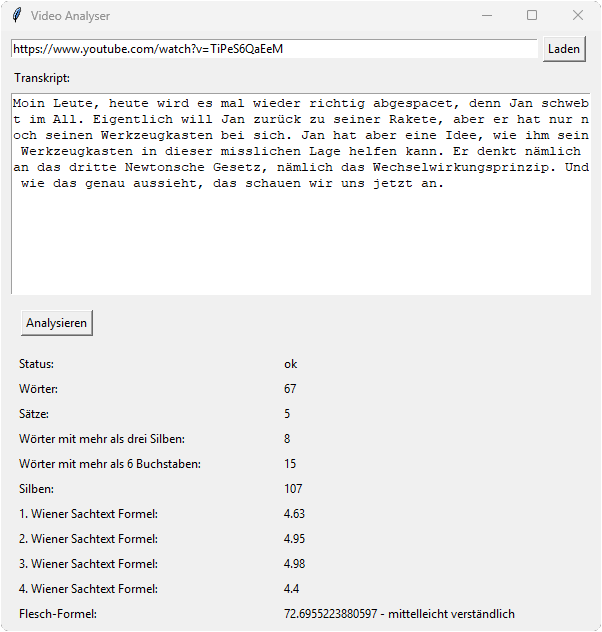
\includegraphics[width=0.8\textwidth]{tool.png}
			\caption{Video-Analyse-Tool} 
		\end{figure}

	\end{mycolumns}
\end{frame}


\section{Analyse und Ergebnisse}
\begin{frame}{\insertsection}
Analyse von Videos von the Simple Club
\begin{itemize}
	\item Thema -- Newtonsche Axiome
	\begin{itemize}
		\item Newtonsche Axiome
		\item Trägheitsprinzip
		\item Aktionsprinzip
		\item Wechselwirkungsprinzip
	\end{itemize}
	\item Analyse mit dem Video-Analyse-Tool
	\item Bildungsplan: Gymnasium, Klasse 7/8 (und 9/10)
\end{itemize}

\begin{figure}
	\centering
	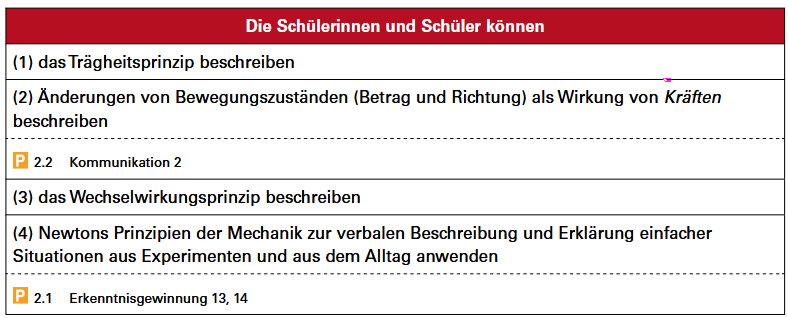
\includegraphics[width=0.6\textwidth]{Bildungsplan327.png}
	\caption{Bildungsplan Gymnasium, BW, Klasse 7/8, \href{https://bildungsplaene-bw.de/\%2CLde/LS/BP2016BW/ALLG/GYM/PH.V2/IK/7-8/07}{https://bildungsplaene-bw.de/}}
	
\end{figure}


\end{frame}


%\subsection{The Simple Club}
\begin{frame}{\insertsection}
\textbf{The Simple Club-Videos:}
	\begin{table}
		\begin{tabular}{|l|c|c|l|c|}
			\hline
			\textbf{Video} & \textbf{WSTF4} & \textbf{FRE}$_{\mathrm{de}}$ & \textbf{Video ID} & Länge (min) \\
			\hline
Newtonsche Axiome & 5.14 & 70.28  & \href{https://www.youtube.com/watch?v=skFzB2nmMwM}{skFzB2nmMwM} & 2.55 \\
			\hline
Trägheitsprinzip  & 4.35     & 72.27 & \href{https://www.youtube.com/watch?v=x04Qgfqo7Bg}{x04Qgfqo7Bg} & 4.50 \\
			\hline
Aktionsprinzip    & 4.92 & 72.42  & \href{https://www.youtube.com/watch?v=g1LfwG2pSs4}{g1LfwG2pSs4} & 5.05 \\
			\hline
Wechselwirkungsprinzip & 5.27 & 67.41  & \href{https://www.youtube.com/watch?v=TiPeS6QaEeM}{TiPeS6QaEeM} & 5.03  \\
			\hline
			\hline
\textbf{Mittelwert} & 4.92  & 70.60 & & 4.38 \\
			\hline
		\end{tabular}
		\caption{Lesbarkeitsindex für The Simple Club}
	\end{table}

	\begin{itemize}
		\item Mittelwert der Lesbarkeitsindex: 4.92 $\Rightarrow$ für Schüler:innen ab Klasse 5 geeignet
		\item im Bildungsplan: Gymnasium, Klasse 7/8 (und 9/10)
		\item Videos von The Simple Club zeichnen sich durch einfache Sprache aus.
	\end{itemize}
	


\end{frame}

% \begin{frame}
% 	\begin{mycolumns}
% \textbf{The Simple Club: Wechselwirkungsprinzip} \\
% \textcolor{orange}{Okay, hier noch ein anderes Beispiel was nicht so abgespact ist:}
% \textcolor{green}{Wenn ein Jäger im Wald mit seinem Gewehr schießt, dann gibt das einen lauten Knall.}
% \textcolor{green}{Klar, aber was passiert da physikalisch im Gewehr?} 
% \textcolor{green}{Das Gewehr übt beim Schuss eine Kraft auf die Kugel aus, diese fliegt davon.} 
% \textcolor{red}{Allerdings entsteht aufgrund des Wechselwirkungsprinzips auch eine Kraft von der Kugel auf das Gewehr, das ist die Gegenkraft.} \textcolor{green}{Diese Kraft ist bei einem Gewehr als Rückstoß bekannt.} \textcolor{red}{Die Gegenkraft ist genauso groß wie die ursprüngliche Kraft die auf Kugel wirkt, außerdem ist sie entgegengesetzt gerichtet.} \textcolor{orange}{Da das Gewehr allerdings viel schwerer ist als die Kugel, erreicht das Gewehr nicht dieselbe Geschwindigkeit wie die Kugel.}


% % 0-4 grün
% % 4-6 orange
% % 6-12 rot
% 		\begin{tabular}{ll}
% 			Sätze: & 8 \\
% 			Wörter: & 112 \\
% 			Silben: & 181 \\
% 			Silben $\geq 3$: & 15 \\
% 			4 WSTF: & 4.94 \\
% 			Flesch-Index: & 70.97 (mittelleicht)\\  
% 		\end{tabular}

% 		\mynextcolumn

% \textcolor{orange}{Die Raumsonde Voyager-1 bewegt sich seit 1977 durch das Weltall.}
% \textcolor{green}{Sie braucht dazu keinen Antrieb. Den Grund dafür kennst du.}
% \textcolor{red}{Es gilt das Trägheitsprinzip:}
% \textcolor{red}{Ohne Einwirkung durch einen anderen Körper bewegt sich ein Körper mit konstanter Geschwindigkeit in die gleiche Richtung weiter.} 
% \textcolor{green}{Mit dem Impuls formuliert heißt das:}  
% \textcolor{red}{Der Impuls eines Körpers bleibt erhalten, solange kein anderer Körper auf ihn einwirkt.}

% \begin{tabular}{ll}
% 	Sätze: & 8 \\
% 	Wörter: & 112 \\
% 	Silben: & 181 \\
% 	Silben $\geq 3$: & 15 \\
% 	4 WSTF: & 4.94 \\
% 	Flesch-Index: & 70.97 (mittelleicht)\\  
% \end{tabular}

% 	\end{mycolumns}
% \end{frame}


\begin{frame}
	\begin{mycolumns}
		\textbf{The Simple Club: Wechselwirkungsprinzip} \\ {\tiny \href{https://www.youtube.com/watch?v=TiPeS6QaEeM}{https://www.youtube.com/watch?v=TiPeS6QaEeM}} \\[1em]
{\footnotesize 
Beim Kräftegleichgewicht wirken zwei entgegengesetzte, gleich große Kräfte auf ein Körper.Das klassisches Beispiel wäre das Seilziehen: Mannschaft 1 zieht das Seil nach links, Mannschaft 2 zieht mit der gleichen Kraft in entgegengesetzte Richtung. Die zwei Kräfte sind gleich groß und heben sich gegenseitig auf. Sie wirken beide auf das Seil und das Seil bewegt sich deshalb nicht, denn die Kräfte heben sich ja auf. Und beim Wechselwirkungsprinzip, da sind die Kräfte ja auch gleich groß und wirken in entgegengesetzte Richtungen. Es gibt aber einen Unterschied und der ist ganz wichtig. Beim Wechselwirkungsprinzip wirkt die eine Kraft von Körper A auf Körper B, die Gegenkraft aber von Körper B auf Körper A. Die zwei Kräfte wirken also nie auf den gleichen Körper. Also zurück zu unserem Jäger. Wenn dieser mit seinem Gewehr schießt, dann übt das Gewehr eine Kraft auf die Kugel aus. Diese wird beschleunigt. Umgekehrt wirkt eine gleichgroße Kraft von der Kugel auf das Gewehr. Diese sind zwar auch entgegengesetzt gerichtet, da sie aber an verschiedenen Körpern angreifen heben sie sich gegenseitig nicht auf.
}


% 0-4 grün
% 4-6 orange
% 6-12 rot

		\mynextcolumn
		\textbf{Universum Physik: Wechselwirkung \& Gleichgewicht} \\
{\tiny Universum Physik BW 9/10 (S. 234)}\\[1em]
{\footnotesize 
Wechselwirkungsgesetz und Kräftegleichgewicht bei zwei Kräften kann man leicht verwechseln. Bei beiden geht es um zwei Kräfte, die gleich groß und entgegengesetzt gerichtet sind. Aber es gibt einen wesentlichen Unterschied. Die Kräfte bei der Wechselwirkung werden auf unterschiedliche Körper ausgeübt: Beim Sitzen übst du eine Kraft auf den Stuhl aus und der Stuhl übt eine Kraft auf dich aus. Beim Kräftegleichgewicht betrachtet man Kräfte, die auf einen Körper ausgeübt werden und sich dabei gegenseitig aufheben: Du bist im Kräftegleichgewicht, weil die Erde dich mit der Gewichtskraft nach unten zieht, aber der Stuhl verhindert, dass du auf den Boden landest.}\\[7em] \



	\end{mycolumns}
\end{frame}

\begin{frame}
	\begin{mycolumns}
\textbf{The Simple Club: Wechselwirkungsprinzip} \\ {\tiny \href{https://www.youtube.com/watch?v=TiPeS6QaEeM}{https://www.youtube.com/watch?v=TiPeS6QaEeM}} \\[1em]
% 0-4 grün
% 4-6 orange
% 6-12 rot
		\begin{tabular}{lrl}
			Sätze:  & 13  & \\
			Wörter: & 172 & (13.23 pro Satz) \\
			Silben: & 284 & (1.65 pro Wort) \\
			Silben $\geq 3$:& 21 & (\textcolor{green}{\textbf{12.21\%}}) \\
			4 WSTF: & \textcolor{green}{\textbf{4.45}}  & (Klassenstufe 5)\\
			Flesch-Index: & 69.68 & (mittel verständlich)\\  
		\end{tabular}

		\mynextcolumn
\textbf{Universum Physik: Wechselwirkung \& Gleichgewicht} \\
{\tiny Universum Physik BW 9/10 (S. 234)}\\[1em]
\begin{tabular}{lrl}
	Sätze: & 7    & \\
	Wörter: & 99  & (14.14 pro Satz) \\
	Silben: & 173 & (1.74 pro Wort) \\
	Silben $\geq 3$: & 19 & (\textcolor{red}{\textbf{19.19\%}}) \\
	4 WSTF: & \textcolor{red}{\textbf{6.69}} & (Klassenstufe 7)\\
	Flesch-Index: & 63.10 & (mittel verständlich)\\  
\end{tabular}
	\end{mycolumns}
	\ \\[2em]
	\begin{definition}{4. Wiener Sachtextformel}
$$G_4 = 0{,}2744 \cdot MS + 0{,}2656 \cdot SL - 1{,}693 $$
	\begin{itemize}
		\item MS: Prozentualer Anteil der Wörter mit drei oder mehr Silben
		\item SL: Durchschnittliche Satzlänge (Anzahl der Wörter pro Satz)
	\end{itemize}
				
\end{definition}
\end{frame}


\begin{frame}
	\begin{mycolumns}
		\textbf{The Simple Club: Wechselwirkungsprinzip} \\ {\tiny \href{https://www.youtube.com/watch?v=TiPeS6QaEeM}{https://www.youtube.com/watch?v=TiPeS6QaEeM}} \\[1em]
{\footnotesize 
Beim \textcolor{red}{Kräftegleichgewicht} wirken zwei \textcolor{red}{entgegengesetzte,} gleich große Kräfte auf ein Körper.Das \textcolor{red}{klassisches} Beispiel wäre das \textcolor{red}{Seilziehen:} Mannschaft 1 zieht das Seil nach links, Mannschaft 2 zieht mit der gleichen Kraft in \textcolor{red}{entgegengesetzte} Richtung. Die zwei Kräfte sind gleich groß und heben sich \textcolor{red}{gegenseitig} auf. Sie wirken beide auf das Seil und das Seil bewegt sich deshalb nicht, denn die Kräfte heben sich ja auf. Und beim \textcolor{red}{Wechselwirkungsprinzip}, da sind die Kräfte ja auch gleich groß und wirken in \textcolor{red}{entgegengesetzte} \textcolor{red}{Richtungen}. Es gibt aber einen \textcolor{red}{Unterschied} und der ist ganz wichtig. Beim \textcolor{red}{Wechselwirkungsprinzip} wirkt die eine Kraft von Körper A auf Körper B, die \textcolor{red}{Gegenkraft} aber von Körper B auf Körper A. Die zwei Kräfte wirken also nie auf den gleichen Körper. Also zurück zu \textcolor{red}{unserem} Jäger. Wenn dieser mit seinem Gewehr schießt, dann übt das Gewehr eine Kraft auf die Kugel aus. Diese wird \textcolor{red}{beschleunigt}. \textcolor{red}{Umgekehrt} wirkt eine \textcolor{red}{gleichgroße} Kraft von der Kugel auf das Gewehr. Diese sind zwar auch \textcolor{red}{entgegengesetzt} \textcolor{red}{gerichtet}, da sie aber an \textcolor{red}{verschiedenen} Körpern \textcolor{red}{angreifen} heben sie sich \textcolor{red}{gegenseitig} nicht auf.
}


% 0-4 grün
% 4-6 orange
% 6-12 rot

		\mynextcolumn
		\textbf{Universum Physik: Wechselwirkung \& Gleichgewicht} \\
		{\tiny Universum Physik BW 9/10 (S. 234)}\\[1em]
{\footnotesize 
\textcolor{red}{Wechselwirkungsgesetz} und \textcolor{red}{Kräftegleichgewicht} bei zwei Kräften kann man leicht \textcolor{red}{verwechseln.} Bei beiden geht es um zwei Kräfte, die gleich groß und \textcolor{red}{entgegengesetzt} \textcolor{red}{gerichtet} sind. Aber es gibt einen \textcolor{red}{wesentlichen} \textcolor{red}{Unterschied.} Die Kräfte bei der \textcolor{red}{Wechselwirkung} werden auf \textcolor{red}{unterschiedliche} Körper \textcolor{red}{ausgeübt:} Beim Sitzen übst du eine Kraft auf den Stuhl aus und der Stuhl übt eine Kraft auf dich aus. Beim \textcolor{red}{Kräftegleichgewicht} \textcolor{red}{betrachtet} man Kräfte, die auf einen Körper \textcolor{red}{ausgeübt} werden und sich dabei \textcolor{red}{gegenseitig} \textcolor{red}{aufheben:} Du bist im \textcolor{red}{Kräftegleichgewicht,} weil die Erde dich mit der \textcolor{red}{Gewichtskraft} nach unten zieht, aber der Stuhl \textcolor{red}{verhindert,} dass du auf den Boden landest.}\\[7em] \



	\end{mycolumns}
\end{frame}


\section{Zusammenfassung}

\begin{frame}{\insertsection}
	\begin{itemize}
		\item The Simple Club laut Wiener Sachtextformeln und Fleschindex einfacher zu verstehen als Schulbücher:
		\begin{itemize}
			\item Prozentualer Anteil der Wörter mit drei oder mehr Silben deutlich geringer.
			\item Einfluss von Satzlänge auf Differenz aufgrund geringer Unterschiede eher gering
			\item The Simple Club Text deutlich länger als Schulbuchtext.
			\item The Simple Club: Klassenstufe 5, Schulbuch: Klassenstufe 7
		\end{itemize}
		\item Zu beachten: 
		\begin{itemize}
			\item Stichprobe für The Simple Club ist klein.
			\item Vergleich mit Schulbüchern ist nicht repräsentativ.
		\end{itemize}
	\end{itemize}
\end{frame}

\end{document}
